% -----------------------------------------------------------------------------
% November, 2023 update by Eve Torrence
% This file contains a sample Bridges paper in LaTeX format.
% The original was written by Carlo S\'equin in 2017, using previous
% versions by Doug McKenna, Craig Kaplan, Reza Sarhangi, and others,
% with \LaTeX\ contributions by Bruce Torrence and David Swart.
% It has been vetted using TeXShop 5.10 on Mac OS Big Sur (11.6).
% TeXShop is part of the TeX Live distribution, available
% at http://www.tug.org/texlive/
%
% -----------------------------------------------------------------------------

\documentclass[letterpaper,11pt]{article}
\usepackage{amsmath, amsthm, amssymb}    % May not all be necessary
\usepackage{bridges}			% Custom bridges proceedings style
\usepackage{graphicx}			% For including pictures
\usepackage[colorlinks=true, urlcolor=blue, citecolor=black, linkcolor=black]{hyperref}  
							% For formatting (clickable) URLs
\usepackage{subcaption}			% For captioning multi-panel figures

\urlstyle{rm} 					% Display URLs in same font as body text

% -----------------------------------------------------------------------------

\title{Simulating Digital Circuits Using Wang Cubes [under construction]}

\author{Mathew Kuthur James\textsuperscript{1}
\vspace{10pt}\\
\textsuperscript{1}David Cheriton School of CS, University of Waterloo} % end \author
% superscripts are only needed if there is more than one author

% \date{[Draft as of \today]}	% uncomment to use for your own draft purposes
\date{}					% Suppress any date on submissions

% -----------------------------------------------------------------------------

\begin{document}

\maketitle

% Prevent page number 1 from being printed on the first page.
\thispagestyle{empty}

\begin{abstract}

This report describes a method by which Wang cubes tiling 3D space can be used to simulate digital circuits, and presents a web-app to run such simulations. It also describes an efficient algorithm used to compute adjacent planes along the z-axis, along with the software architecture and technology used to create the web-app. Common elements of digital circuits (such as clocks, wires, logic gates, \emph{et cetera}), along with the challenges of instantiating them using Wang cubes, are discussed here.

\end{abstract}

% Bridges papers are usually no more than 8 pages in length.  So
% there's really no need to have numbered sections, unless the
% author really needs to refer to sections by number within the paper's text.  
% So to suppress sequential section numbers, append an asterisk to 
% the \section command, as in:

\section*{Introduction}

The primary goal of this project is to develop software to design and tile $R^3$ with Wang cubes, which are the 3D analogue for Wang tiles. Since 2D Wang tiles are Turing-complete, 3D Wang tiles possesses the expressive power required to simulate a Von Neumann machine built out of simple circuit elements like clocks, wires, logic-gates and flip-flops. 

Movement along the z-axis is treated as equivalent to stepping forward and backward in time, which is treated as a distinct quantity. At each stage, the current plane contains a finite number of tiles, which are used to compute the preceding and succeeding plane in real time. The algorithm to do so is described in this report. A user manual \cite{manual}, the web-app \cite{web-app}, its source \cite{web-app-source} and files describing common circuit elements \cite{wang-file} are available online.


\section*{Architecture}

\begin{figure}[h!tbp]
	\centering
	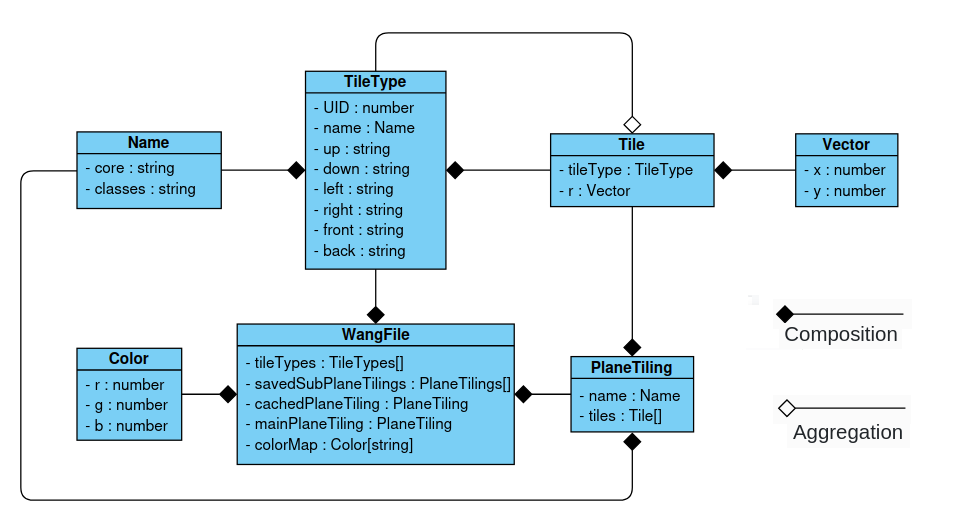
\includegraphics[width=6.4in]{figures/class-diagram.png}
	\caption{A UML class diagram describing the ontology underlying the system}
	\label{fig:1}
\end{figure}

A "tile type" refers to an entity that describes the adjacency rules which determine the legality of a tiling. A tile is a combination of a tile type with a position vector (a vector being a 2-tuple of real numbers). All tiles have positions which are aligned with the grid - each number in the 2-tuple is an integer.

A tiling is a collection of tiles in the x-y plane. The function mapping the tiles in a plane tiling to the set of tile types is surjective, but not necessarily injective. The function mapping the tiles in a tiling to the set of all possible positions is surjective, and not injective (since there are an infinite possible number of positions, and the number of tiles is finite).


Instead of using colors, the adjacency rules for tiles are enforced using strings. A significant advantage of using unicode strings instead of RGB 3-tuples is that a string is self-documenting. Another advantage is that strings are easy to tell apart from each other, unlike close shades of colors. Furthermore, the system is designed such that one can use it even if completely color-blind, albeit not as efficiently as if one can perceive colors perfectly.

A Wang file consists of a global set of tile types, a main tiling (on which most of the work is done), a cached tiling (used to implement resets while editing), a collection of sub tilings (which can be copied from and pasted into the main plane tiling) and a global color map that maps strings to colors. 

The entire state of the data is stored in the Wang file, and the Wang file can be exported and imported via JSON \cite{json} serialization. This process presents the following challenges:


\begin{itemize}
	\item JSON objects do not preserve references, so if multiple tiles have references to the same tile type object, deserialization creates two distinct but identical tile type objects. This is resolved using a readonly static UID associated with the tile type class, which is used to collapse references to identical tile types into a single object. 
	\item JSON objects carry only data and do not record non-static functions. This is resolved by replacing all non-static functions with static functions bound to the class, that takes an additional argument in place of "this" that the non-static function operates on.
	
\end{itemize}

\section*{Algorithm}

Given n tiles and m tile-types, a naïve backtracking algorithm operates with a time complexity of $O(m^n)$, which is unsuitable for Wang files which use many different tile types. Thus, a more efficient algorithm is used.

The computation of the neighboring planes is done using PRUNE (Propagation and Reduction Using Neighborhood Elimination), which is a modification of the wave-function collapse algorithm \cite{Merrel}. PRUNE requires that the current plane can have exactly one possible adjacent plane. Tilings that are non-deterministic are not supported, and the exact point of where the non-determinism occurs is pointed out by PRUNE.

The high-level idea behind PRUNE is:

\begin{itemize}
	\item Each tile has a set of possible tile types that its neighbor in the next plane can have.
	\item Given a pair of tiles, the set of possible tile types of one tile can be reduced by considering the set of possible tile types of the other tile.
	\item A pass consists of applying a reduction to every pair of adjacent tiles in the tiling.
	\item PRUNE makes multiple passes, and terminates when a reduction-free pass is made.
	\item If a pass does not allow any reductions to be made, no further passes result in any reductions (since none of the sets of possible tile types are changed, making the result of every subsequent pass the same)
\end{itemize}

An analysis of the algorithm's correctness and efficiency is presented below:

\begin{itemize}
	\item The maximum cardinality of the set of possible tile types is m.
	\item Let $I$ be the sum of cardinalities of the set of possible tile types of every tile. Since there are n tiles, $I \leq mn$
	\item Let $I_k$ be the value of $I$ at the $k^{\text{th}}$ pass.
	\item Since no pass expands the possible tile types, $I_{k+1} \leq I_k$
	\item If a pass does result in a reduction, at least one set of possible tile-types is reduced in size. Thus, $I_{k+1} < I_k$
	\item Thus, the maximum number of passes before termination is $mn$. Since each pass takes $O(n)$ time, the overall complexity of the algorithm is $O(mn^2)$
\end{itemize}

Thus, PRUNE uses repeated passes and computes the plane in $O(mn^2)$ time, which is significantly faster than the naïve backtracking approach. However, since the data structures that store tiles do not store the neighbors of the tiles, generating a neighbor-graph requires $O(n^2)$ preprocessing time and $O(n)$ space, which is the overhead for the current implementation of PRUNE. Maintaining a live neighbor-graph with each edit allows the preprocessing time to disappear entirely, when amortization is accounted for.


\section*{Technology}

The software was designed to be a web-app, since this would allow it to be used by anyone with a browser. This also saves a lot of developer effort that would otherwise be spent in packaging the software for various operating systems and platforms.

\begin{figure}[h!tbp]
	\centering
	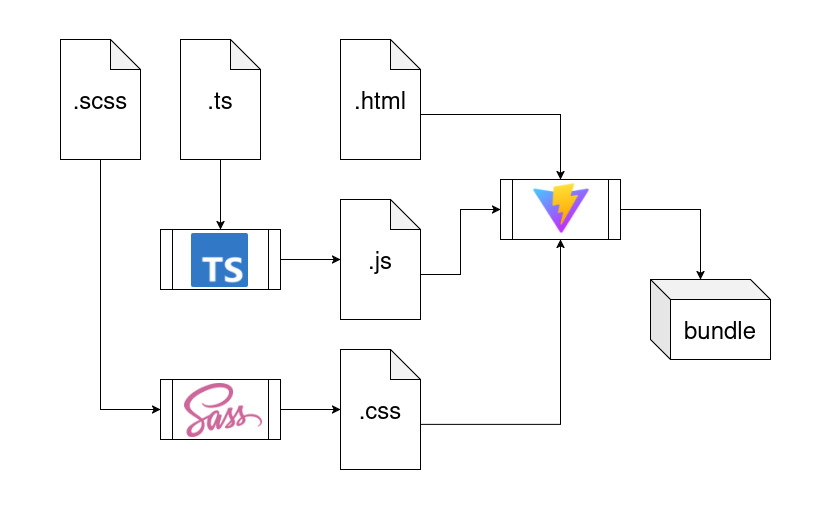
\includegraphics[width=6.4in]{figures/pipeline.png}
	\caption{The build pipeline, from the source files to the bundle}
	\label{fig:2}
\end{figure}

The following technology was used in the web-app:

\begin{itemize}
	\item HTML5 \cite{HTML5}, which is the industry standard for web development, used for the high-level structure of the web-app
	\item NPM \cite{npm} (Node package manager), used to install and maintain dependencies
	\item SASS \cite{sass} (Syntactically Awesome StyleSheets), which is a superset of CSS with additional syntactic sugar, used for styling the elements of the web-app
	\item TypeScript \cite{typescript}, which is a superset of JavaScript with a typing system, used for the describing the algorithms, data structures and UI interactions of the web-app
	\item three.js \cite{3js}, a package used to render objects in 3D using a WebGL context, without having to write any WebGL code directly
	\item Vite \cite{vite}, used to manage the compilation to CSS/JavaScript, minification \cite{minification}, tree-shaking \cite{tree} and bundling the web-app into a small, portable form
	\item Vitepress \cite{vitepress}, a static site generator \cite{ssg} used to generate the user manual from markdown \cite{markdown} source files
	\item GitHub actions, used as a CI/CD solution to build and publish the web-app incrementally
	\item GitHub pages, used to host the web-app online
\end{itemize}

In addition, the icons for the web-app were sourced from Google Material \cite{google-material} icons, downloaded as SVG images.


\section*{Results}

A reference implementation for a two-state standalone clock is described below:

\begin{table}[h!tbp]
	\centering
	\caption{Adjacency rules for standalone-clock-0}
	{\footnotesize % reduce the font size for entire table
	\begin{tabular}{|l|r|}
	\hline
	  string & value \\
	\hline
	up & anything \\
	\hline
	down & anything \\
	\hline
	left & anything \\
	\hline
	right & anything \\
	\hline
	front & clock-1 \\
	\hline
	back & clock-0 \\
	\hline
	\end{tabular}
	}
	\end{table}

	\begin{table}[h!tbp]
		\centering
		\caption{Adjacency rules for standalone-clock-1}
		{\footnotesize % reduce the font size for entire table
		\begin{tabular}{|l|l|}
		\hline
		  string & value \\
		\hline
		up & anything \\
		\hline
		down & anything \\
		\hline
		left & anything \\
		\hline
		right & anything \\
		\hline
		front & clock-0 \\
		\hline
		back & clock-1 \\
		\hline
		\end{tabular}
		}
		\end{table}

The standalone clock consists of two states - clock-0 and clock-1. Each state only allows the other state to be placed next to it in the plane behind and in front of it along the z-axis. When moving along the z-axis, the tile at that location alternates between clock-0 and clock-1, which simulates a clock pulse.

\begin{figure}[h!tbp]
	\centering
	\begin{minipage}[b]{0.2\textwidth} 
		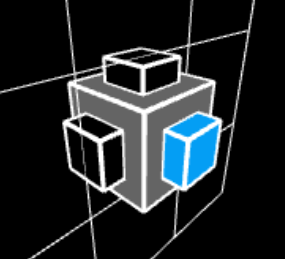
\includegraphics[width=\textwidth]{figures/0-clock.png}
				\subcaption*{standalone-clock-0} % Add subcaption text if desired, or use \subcaption* to suppress (a), (b), etc. labels
				\label{fig:2a}
	\end{minipage}
	~ %add desired spacing between images, e. g., ~, \quad, \qquad, \hfill etc.	
	\begin{minipage}[b]{0.2\textwidth} 
		
\includegraphics[width=\textwidth]{figures/1-clock.png}
				\subcaption*{standalone-clock-1} % Add subcaption text if desired, or use \subcaption* to suppress (a), (b), etc. labels
				\label{fig:2b}
	\end{minipage}
	\caption{standalone-clock: "clock-0" is mapped to grey and "clock-1" is mapped to cyan}
	\label{fig:2}
	\end{figure}


	Clocks that have different frequencies are implemented by adding more states - for instance, a clock that runs at half the base frequency has 4 states - clock-00, clock-01, clock-10 and clock-11. Other elements that don't have internal states that depend directly on time are given adjacency rules such that they propagate themselves.

	\begin{table}[h!tbp]
		\centering
		\caption{Adjacency rules for horizontal-wire-0}
		{\footnotesize % reduce the font size for entire table
		\begin{tabular}{|l|r|}
		\hline
		  string & value \\
		\hline
		up & anything \\
		\hline
		down & anything \\
		\hline
		left & 0 \\
		\hline
		right & 0 \\
		\hline
		front & wire \\
		\hline
		back & wire \\
		\hline
		\end{tabular}
		}
		\end{table}
	
		\begin{table}[h!tbp]
			\centering
			\caption{Adjacency rules for horizontal-wire-1}
			{\footnotesize % reduce the font size for entire table
			\begin{tabular}{|l|l|}
			\hline
			  string & value \\
			\hline
			up & anything \\
			\hline
			down & anything \\
			\hline
			left & anything \\
			\hline
			right & anything \\
			\hline
			front & wire \\
			\hline
			back & wire \\
			\hline
			\end{tabular}
			}
			\end{table}

For all such elements, rotations and reflections require different tile types, though the relationships between the adjacency rules of rotated and reflected tile types enables the web app to generate them automatically, without requiring the user to manually enter all the rules.

\begin{figure}[h!tbp]
	\centering
	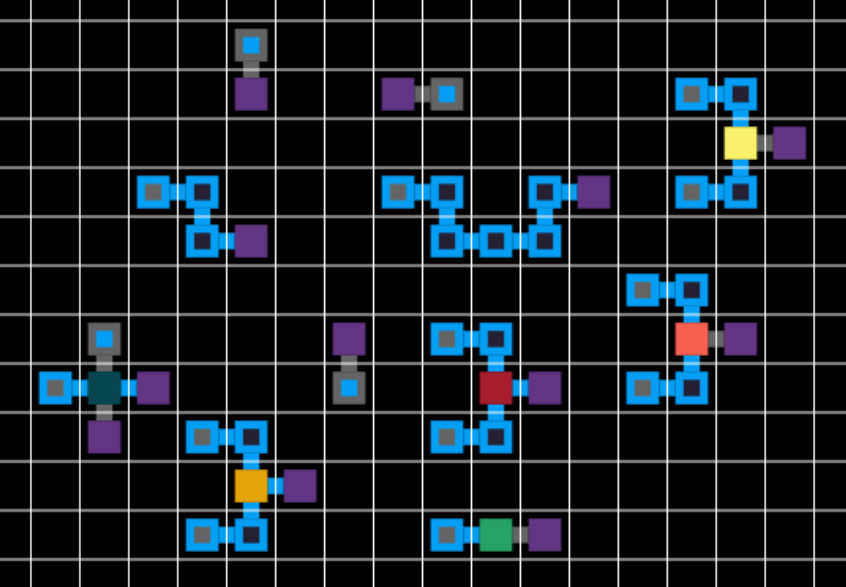
\includegraphics[width=6.4in]{figures/gates-wires-clocks.png}
	\caption{Logic gates: AND (red), OR (deep-yellow) NOT (green), NAND (orange), NOR (light-yellow), wires (grey/cyan), junctions (deep cyan), clocks,  and sinks (purple)}
	\label{fig:2}
\end{figure}


\section*{Future work}

The following circuits can be added to the project:

\begin{itemize}
	\item D-flip-flops, constructed either as a standalone tile or from two D-latches. This requires a consistent translation of the notion of rising and falling edges to a system with discrete time, which requires research into variants of flip-flops
	\item shift-registers, built from T-flip-flops. This allows one to build clocks of arbitrary frequencies without creating a large number of clock tiles to represent each state
	\item Single-tile wires with more than two states, which can be used to transmit signals effectively, when coupled with multiplexers and demultiplexers
	\item A 7-segment display, using a $3 x 5$ grid of screen tiles, with each tile having 10 states, though making 150 manually using the current UI is tedious
\end{itemize}

The following UI improvements can be made to the project:

\begin{itemize}
	\item An implementation of the pause/play functionality, which is currently left unimplemented due to difficulties involved with managing the animation framerate with the system clock (for security reasons, most browsers do not allow scripts to access the exact time on the system clock)
	\item A custom console, to display errors and warnings at different levels of verbosity (at present, all such messages show up in the console provided with the developer tools of the browser)
	\item An input console to allow the programmatic manipulation of the Wang file, to automate tedious tasks
	\item Collapsible classes in the search results, making a tree-like structure that's easier to navigate than scrolling over all the results
	\item A graphical representation of the illegality of the tiling (for instance, using red circles to point out areas where the adjacency rules are violated)
	\item Integrating the main editor with three.js, allowing the user to manipulate the main tiling using orbit controls (currently unimplemented due to problems with mixing dynamic resizing with the WebGL API of three.js)
\end{itemize}

\section*{LLM disclosure}

No LLMs were used in the generation of this report or the user manual for the web-app. However, when writing the code for the web-app, the involvement of LLMs is difficult to quantify and disentangle from the code written by a human, for the following reasons:

\begin{itemize}
	\item Development often involves copying and pasting code from online forums such as StackOverflow. The source of the content on such forums cannot be guaranteed to be written by a human, unless accompanied with a timestamp preceding the release of popular LLMs like ChatGPT.
	\item Since search engines integrate AI assistance with their service, searching for a topic results in the user being exposed to an AI-generated answer that appears before every search result. This could subtly influence the thought-process of the user, guiding them toward certain implementations and solutions.
	\item Popular code-editors like Copilot now integrate agentic coding assistants powered by LLMs, which autocomplete code snippets and generate functions from comments. Though no such editor has been used in the development of this web-app, it is often the case that the coder does not have direct control over what editor they are allowed to use.
\end{itemize}


%%%%%%%%%%%%%%%%%%%%%%%%%%%%%%%%%%%%%%%
\section*{Acknowledgements}

The author would like to acknowledge the attendees of CS898 Spring 2025, for their feedback on features to implement in the web-app.

%%%%%%%%%%%%%%%%%%%%%%%%%%%%%%%%%%%%%%
% References %
    
{\setlength{\baselineskip}{13pt} % tighten line spacing for bibliography
\raggedright				% no right justification for References
\begin{thebibliography}{99}

% \bibitem{Chang}
% W. Chang. \LaTeX\ \textit{Cheat Sheet}. 2014. \url{http://wch.github.io/latexsheet/}.

% \bibitem{EJCx}
% M.\ Chladn\'y and M.\ \v Skoviera. ``Factorisation of Snarks.'' \textit{Electronic Journal
% of Combinatorics}, vol.~17, no.~1, R32, 2010.
% \url{http://www.combinatorics.org/Volume_17/PDF/v17i1r32.pdf}.

% \bibitem{Coxeter} H.\ S.\ M.\ Coxeter. ``The Non-Euclidean Symmetry of Escher's Picture
% Circle Limit III.'' \textit{Leonardo}, vol.~12, no.~1, 1979, pp.~19--25.

% \bibitem{easychair} EasyChair. Log in page. \url{https://easychair.org/account/signin.cgi}.

% \bibitem{Gratzer} G.\ Gr\"atzer. \textit{More Math Into} \LaTeX, 4th ed. Springer, 2007.

% \bibitem{Sequin2016} C.\ H.\ S\'equin. ``From Klein Bottles to Modular Super-Bottles.'' 
% \textit{Bridges Conference Proceedings}, Jyv\"askyl\"a, Finland, Aug. 9--13,
% 2016, pp.~41--48. \url{http://archive.bridgesmathart.org/2016/bridges2016-41.html}.


\bibitem{manual} User manual, GitHub pages. \url{https://mathewkj2048.github.io/Wang-cube-circuit-simulator-user-manual}

\bibitem{web-app} Web app, GitHub pages. \url{https://mathewkj2048.github.io/Wang-cube-circuit-simulator/}

\bibitem{web-app-source} Web app source code, GitHub \url{https://github.com/MathewKJ2048/Wang-cube-circuit-simulator}

\bibitem{wang-file} Clocks, wires and logic gates, GitHub \url{https://github.com/MathewKJ2048/Wang-cube-circuit-simulator/tree/main/Wang-files}

\bibitem{Merrel} Merrel, Paul. ``Example-based model synthesis'' \textit{Proceedings of the 2007 Symposium on Interactive 3D Graphics and Games}, 2007, pp.105--112 \url{https://doi.org/10.1145/1230100.1230119}

\bibitem{tree} Tree-shaking, MDN web docs. \url{https://developer.mozilla.org/en-US/docs/Glossary/Tree_shaking}

\bibitem{minification} Minification, MDN web docs. \url{https://developer.mozilla.org/en-US/docs/Glossary/Minification}

\bibitem{HTML5} HTML5,  MDN web docs. \url{https://developer.mozilla.org/en-US/docs/Glossary/HTML5}

\bibitem{sass} Documentation, sass-lang. \url{https://sass-lang.com/documentation/}

\bibitem{typescript} TypeScript,  MDN web docs. \url{https://developer.mozilla.org/en-US/docs/Glossary/TypeScript}

\bibitem{vite} Vite. \url{https://vite.dev/}

\bibitem{ssg} Static Site Generator, MDN web docs. \url{https://developer.mozilla.org/en-US/docs/Glossary/SSG}

\bibitem{npm} Node Package Manager. \url{https://docs.npmjs.com/about-npm}

\bibitem{markdown} How to write in Markdown, MDN web docs. \url{https://developer.mozilla.org/en-US/docs/MDN/Writing_guidelines/Howto/Markdown_in_MDN}

\bibitem{json} JavaScript Object Notation. \url{https://www.json.org/json-en.html}

\bibitem{vitepress} Vitepress \url{https://vitepress.dev/}

\bibitem{3js} three.js \url{https://threejs.org/}

\bibitem{google-material} Google Material icons. \url{https://fonts.google.com/icons}



\end{thebibliography}
} % end setlength, raggedright
   
\end{document}